\documentclass[]{article}

\usepackage[letterpaper]{geometry}
\usepackage{titlesec}
\usepackage{enumitem}
\usepackage{hyperref}
\usepackage{tabularx}
\usepackage{titling}
\usepackage{framed}
\usepackage{float}
\usepackage{geometry}
\usepackage{tikz}
\usepackage{graphicx}

\usetikzlibrary{decorations.pathmorphing, shapes.geometric, shapes.misc, calc, arrows, arrows.meta, positioning, fit}

\tikzstyle{block} = [rectangle, draw, fill=blue!20, text width=5em, text centered, rounded corners, minimum height=4em]
\tikzstyle{line} = [draw, -latex']
\tikzstyle{cloud} = [draw, ellipse,fill=red!20, node distance=3cm, minimum height=2em]

\setlength{\droptitle}{-5\baselineskip} % Remove space above the title

\title{Empowering Education in the Digital Age: Leveraging Large Language Models for Personalized Learning}
\author{}
\date{}

\begin{document}
\maketitle

\vspace{-4\baselineskip} % Remove four lines worth of space between title and authors

\begin{center}
\begin{tabularx}{\textwidth}{@{}>{\centering\arraybackslash}X@{\quad}>{\centering\arraybackslash}X@{\quad}>{\centering\arraybackslash}X@{}}
\textbf{Bibi Nur Muhamad} & \textbf{Elijah Kulpinski} & \textbf{Fernando Vargas} \\
nurmu001@rangers.uwp.edu & kulpi001@rangers.uwp.edu & varga051@rangers.uwp.edu \\
University of Wisconsin - Parkside & University of Wisconsin - Parkside & University of Wisconsin - Parkside \\
Kenosha, WI, USA & Kenosha, WI, USA & Kenosha, WI, USA \\
\end{tabularx}
\end{center}

\vspace{1\baselineskip} % Add one line worth of space between authors and abstract

\begin{framed}
\begin{abstract}
This proposal seeks to address the challenges posed by traditional educational tools, which often fall short in meeting the evolving needs of modern students in the digital age. Our research focuses on enhancing student critical thinking and engagement in computer science course education, encompassing discussions, quizzes, lectures, homework, and related activities. The core issue at hand is the limited accessibility and engagement associated with conventional educational resources within the computer science domain.

In response to this challenge, we advocate for the application of modern language models, particularly Large Language Models (LLMs), as a valuable tool for teachers rather than a replacement. LLMs have the capacity to revolutionize computer science education by offering dynamic, interactive, and highly personalized learning experiences. Unlike traditional teaching methods, LLMs can be used by teachers to provide students with immediate and precise responses to their questions, creating an engaging learning environment. This innovative approach enables the implementation of one-on-one teaching, a level of personalization that has historically been unfeasible with non-LLM-based teaching solutions within the computer science curriculum.

Our methodology includes the careful supervised fine-tuning of our LLM, ensuring domain-specificity and up-to-date knowledge within the field of computer science. Fine-tuned LLMs have the potential to significantly enhance student critical thinking and engagement by providing teachers with a tool to offer tailored support in discussions, quizzes, lectures, and homework. Teachers can employ LLMs to engage students in conversations, giving them questions tailored to their subject and providing hints as needed, while collecting the resulting interactions. Our team's commitment lies in adapting educational content to cater to the unique needs and preferences of individual computer science learners, thus enhancing the accessibility and engagement of education in the digital age and promoting critical thinking in the context of computer science education.
\end{abstract}
\end{framed}

\vspace{1\baselineskip} % Add one line worth of space between abstract and keywords

\noindent\textbf{Keywords:} Large Language Models (LLMs), Computer Science Education, Personalized Learning, Critical Thinking, Engagement, Education Technology, Data Privacy, Digital Divide, Ethical Considerations, Policy Initiatives, AI in Education, Educational Equity, Education Access, Technology in Learning, Effective Instruction, Business Impacts, Societal Implications, Educational Technology, Educational Innovation, Fine-Tuning, Domain-Specificity, Adaptive Learning, Student Engagement, Educational Content, AI in Teaching, Pedagogy, Educational Resources, One-on-One Teaching, Student-Centric Learning, Educational Enhancement, Digital Age Education.

\section{Motivation: Business, Society, Ethics}

In an era where technology dictates progress, the caliber of education is a prime factor in determining a nation's prosperity, with computer science education at the forefront. This section delineates the drivers behind our research, underscoring the significance of computer science education and its broad impacts on business, society, and ethical practices, thus underscoring the necessity for enhancement.

\subsection{Relevance to Business}

The current business paradigm necessitates a workforce proficient in computer science as the digital transformation reshapes industry norms. This demand has instigated a surge in the need for advanced computer science education, which not only furnishes a skilled workforce but also fosters innovation, fuels technological advancements, and stimulates economic vitality. A case in point is the ACM's findings that businesses thriving on a highly skilled technical workforce are at the vanguard of pioneering innovation and securing a competitive market stance\footnote{\url{https://www.acm.org/}}. Thus, the infusion of advanced computer science education into the labor market is a catalyst for business acumen and growth.

\subsection{Societal and Ethical Implications}

The societal impact of computer science education is manifold, with the power to narrow the digital divide by equipping individuals with vital competencies to partake in the burgeoning digital economy. On the flip side, a deficiency in such education perpetuates socio-economic imbalances. The advent of technologies like LLMs in educational realms brings forth ethical quandaries, including data privacy, the equitable distribution of knowledge, and the responsible use of AI. The ethical implications are illustrated by instances where AI in education has been critiqued for reinforcing biases, thereby amplifying the necessity for ethical vigilance in technology deployment.

\subsection{Political and Policy Considerations}

The interplay between politics and education is pronounced, with government strategies significantly impacted by the demand for advanced computer science education. Recognizing the vital role of technology in future-proofing societies, policy architects have been pivotal in instigating enhancements in computer science education at both federal and state echelons. Recent initiatives across the globe underscore a collective ambition to furnish citizens with the requisite skills to navigate and succeed in the digital age.

\subsection{Conclusion of the Section}

To encapsulate, the impetus for our investigation is embedded in the intricate relevance of computer science education to the economic, societal, and ethical landscape. The burgeoning demand for tech-savvy professionals, the societal benefits of equitable education, the ethical imperatives of AI in pedagogy, and the policy-driven initiatives coalesce to accentuate the exigency and transformative potential of our research. Deciphering these motivations is pivotal to fathoming the scope and impact of our work, poised to redefine education in the digital epoch.

\section{Technology}

\subsection{Introduction to Vocabulary}

To facilitate a thorough understanding of the research technology, we elucidate the following pivotal terms:

1. \textbf{``Large Language Models (LLMs)''}\cite{aisera-llms}: LLMs are sophisticated AI systems capable of comprehending and producing text with human-like nuance. Their ability to process natural language on a vast scale renders them integral to various applications, particularly in education.

2. \textbf{``Supervised Fine-Tuning''}\cite{microsoft-fine-tuning}: A process where a pre-existing model is trained on a domain-specific dataset, supervised fine-tuning enhances the model's acumen for specific tasks.

3. \textbf{``Data Privacy''}\cite{linkedin-dataprivacy}: The safeguarding of personal and sensitive data, which is paramount in educational AI applications to protect student information.

4. \textbf{``Digital Divide''}\cite{soeonline-digitaldivide}: This term refers to the disparities in access to technology and the internet across different socioeconomic groups, impacting educational equity.

5. \textbf{``Ethical Considerations''}\cite{barrage-ethics}: These involve the moral principles guiding AI's educational use to ensure the wellbeing of learners and teachers.

6. \textbf{``Natural Language Processing (NLP)''}\cite{Deslauriers}: A branch of AI focused on the interaction between computers and human language, NLP enables machines to read and interpret human language in a meaningful way.

7. \textbf{``Generative AI''}\cite{Cozzolino}: AI systems that can generate new content by learning from a large corpus of data, often used in the context of generating text, images, or music that resemble human-created content.

8. \textbf{``Few-Shot Learning''}\cite{Zhu}: The ability of a model to learn and generalize from a very small amount of data, which is particularly challenging in machine learning.

9. \textbf{``Sequence-to-Sequence Models''}\cite{Yu}: A class of deep neural network architectures that are designed to convert sequences from one domain to sequences in another domain, often used in translation services and chatbots.

10. \textbf{``Transfer Learning''}\cite{Guo}: A machine learning method where a model developed for a task is reused as the starting point for a model on a second task, leveraging pre-learned patterns for new, related tasks.

\subsection{Technology Description}

Our research delves into an array of peer-reviewed technical and scholarly documents to underpin our understanding of the pertinent technology:

1. \textbf{``Transformers: Novel Neural Network Architectures for Language Understanding''}\cite{Chen}: Transformers, the underlying architecture for state-of-the-art language models like GPT-3, revolutionize how machines handle language by focusing on the relationships between all words in a sentence, regardless of their position.

2. \textbf{``GPT-3: Language Models are Few-Shot Learners'' by Brown et al. (2020)}\cite{MeyerJ}: This paper elaborates on the architecture and capabilities of GPT-3, a prominent LLM celebrated for its few-shot learning abilities, which has significantly influenced adaptive AI in education.

3. \textbf{``Fine-Tuning Pretrained Language Models: Weight Initializations, Data Orders, and Early Stopping'' by Raffel et al. (2019)}\cite{raffel2019finetuning}: This work examines fine-tuning techniques for pretrained language models, highlighting strategies to refine domain-specific performance.

4. \textbf{``The Ethics of Artificial Intelligence in Higher Education'' by Hilton (2019)}\cite{hilton2019ethics}: Hilton investigates the ethical challenges of AI in higher education, exploring issues such as privacy, bias, and equality.

5. \textbf{``E-Learning and the Science of Instruction'' by Clark and Mayer (2016)}\cite{clarkmayer2016elearning}: This resource scrutinizes effective e-learning principles and the role of AI in enhancing pedagogical design and learning outcomes.

6. \textbf{``OpenAI's GPT-3.5: Advancements in Language Comprehension and Generation''}\cite{Ding}: An examination of GPT-3.5 and its innovative capabilities in producing contextually relevant and nuanced text, marking a leap forward in LLMs.

7. \textbf{``Natural Language Understanding in the Age of Deep Learning''}\cite{Mohamadi}: An exploration of the progress in NLP as deep learning models achieve unprecedented understanding of language nuances.

8. \textbf{``Generative AI: The Future of Creative Machines''}:\cite{Göpfert} A study into how generative AI is pushing the boundaries of creativity and the potential implications for automated content creation.

9. \textbf{``Few-Shot Learning: Bridging the Data Gap in AI''}\cite{MeyerJ}:: A comprehensive look at how few-shot learning models are being designed to perform tasks with limited input data, reflecting the future direction of AI research.

10. \textbf{``Sequence-to-Sequence Learning with Neural Networks''}\cite{hilton2019ethics}: Insight into the development of seq2seq models and their impact on tasks that require an understanding of the sequence, such as translation and summarization.

These sources, collectively, provide a broad perspective on the technological advancements and their application in the educational sphere, ensuring that our research is anchored in a deep and current understanding of the field.

\section{Methodology}
\label{sec:methodology}
The methodology of our research hinges on the fine-tuning of Large Language Models (LLMs) to foster a more interactive and constructive educational environment. We have crafted a multistage process that synergizes data processing, LLM training, and conversation modeling. Each stage is underpinned by rigorous academic and practical considerations, ensuring that the fine-tuned LLM can effectively elevate the role of educators by enhancing student learning experiences. The process is detailed as follows:

\subsection{Textbook Conversion to XML}
The conversion of textbooks to XML was initially attempted using regex patterns. However, the lack of consistency in the textbooks' structure led to the decision to manually convert a subset of textbooks to ensure high-quality XML data. This approach, while more resource-intensive, provided a more reliable foundation for subsequent stages of data processing as demonstrated in the following Figures.

\begin{figure}[htbp]
\textbf{\large Converting PDFs to XML}
\centering
\begin{tikzpicture}[auto, node distance=2cm and 2cm, thick,>=Stealth, scale=0.9, every node/.style={transform shape}]
  % Define styles
  \tikzstyle{startstop} = [rectangle, rounded corners, minimum width=3cm, minimum height=1cm,text centered, draw=black, fill=red!30]
  \tikzstyle{io} = [trapezium, trapezium stretches=true, trapezium left angle=70, trapezium right angle=110, minimum width=3cm, minimum height=1cm, text centered, draw=black, fill=blue!30]
  \tikzstyle{process} = [rectangle, minimum width=3cm, minimum height=1cm, text centered, draw=black, fill=orange!30]
  \tikzstyle{decision} = [diamond, aspect=3, minimum width=3cm, minimum height=1cm, text centered, draw=black, fill=green!30]
  \tikzstyle{failure} = [rectangle, minimum width=3cm, minimum height=1cm, text centered, draw=black, fill=pink!70]
  \tikzstyle{arrow} = [thick,->,>=stealth]
  \tikzstyle{line} = [draw, -latex']
  
  % Place nodes
  \node [startstop] (start) {Start Conversion Process};
  \node [io, below of=start] (loadpdfs) {Load PDF Files};
  \node [process, below of=loadpdfs] (extracttext) {Extract Text from PDF};
  \node [process, below of=extracttext] (cleantext) {Clean Extracted Text};
  \node [process, below of=cleantext] (extractmetadata) {Extract Metadata from Text};
  \node [process, below of=extractmetadata] (extractparagraphs) {Extract Paragraphs from Text};
  \node [failure, right=of extractparagraphs] (issue) {Inconsistent Results / Failure Point};
  \node [process, below of=issue] (attemptOCR) {Attempt OCR Conversion};
  \node [process, below of=extractparagraphs] (createXML) {Create XML Structure};
  \node [io, below of=createXML] (writetoXML) {Write to XML File};
  \node [startstop, below of=writetoXML] (finish) {Finish Conversion Process};
  
  % Draw edges
  \path [line] (start) -- (loadpdfs);
  \path [line] (loadpdfs) -- (extracttext);
  \path [line] (extracttext) -- (cleantext);
  \path [line] (cleantext) -- (extractmetadata);
  \path [line] (extractmetadata) -- (extractparagraphs);
  \path [line] (extractparagraphs) -- (createXML);
  \path [line] (createXML) -- (writetoXML);
  \path [line] (writetoXML) -- (finish);
  \path [line] (extractparagraphs.east) -- (issue.west);
  \path [line] (issue) -- (attemptOCR);

  % Key (Legend) for the flowchart
  \node [right=11cm of start, font=\bfseries\large] (keyLabel) {Key};
  \node [startstop, below=0.5cm of keyLabel] (keyStartStop) {Start/Stop Node};
  \node [io, below=0.5cm of keyStartStop] (keyIO) {Input/Output Node};
  \node [process, below=0.5cm of keyIO] (keyProcess) {Process Node};
  \node [failure, below=0.5cm of keyProcess] (keyFailure) {Failure Node};
  \node [decision, below=0.5cm of keyFailure] (keyDecision) {Decision Node};

  % Create a dummy node for positioning the arrow
  \node [below=0.5cm of keyDecision] (dummy) {};
  % Draw an arrow for the key
  \draw [arrow] ([xshift=-10pt]dummy.west) -- ([xshift=10pt]dummy.east);
  % Create a node for the label centered below the arrow
  \node [below=0.1cm of dummy] (arrowLabel) {Flow Direction};
  % Draw a rectangle around the key
  \node [draw, very thin, gray, fit=(keyLabel) (keyStartStop) (keyIO) (keyProcess) (keyDecision) (dummy) (arrowLabel), inner sep=7.5pt] (keyBox) {};

\end{tikzpicture}
\caption{Visual Representation of the Transition from an Initial Text Extraction Process to an OCR Methodology, Highlighting the Point of Inconsistency and the Subsequent Shift in Approach.}
\label{fig:transition_extraction_to_ocr}
\end{figure}

\begin{figure}[htbp]
\textbf{\large Converting PDFs to Markdown to XML Using OCR}
\centering
\begin{tikzpicture}[auto, node distance=2cm and 2cm, thick,>=Stealth, scale=1.0, every node/.style={transform shape}]
  % Define styles
  \tikzstyle{startstop} = [rectangle, rounded corners, minimum width=3cm, minimum height=1cm,text centered, draw=black, fill=red!30]
  \tikzstyle{io} = [trapezium, trapezium stretches=true, trapezium left angle=70, trapezium right angle=110, minimum width=3cm, minimum height=1cm, text centered, draw=black, fill=blue!30]
  \tikzstyle{process} = [rectangle, minimum width=3cm, minimum height=1cm, text centered, draw=black, fill=orange!30]
  \tikzstyle{failure} = [rectangle, minimum width=3cm, minimum height=1cm, text centered, draw=black, fill=pink!70]
  \tikzstyle{arrow} = [thick,->,>=stealth]
  \tikzstyle{line} = [draw, -latex']

  % Place nodes
  \node [startstop] (start) {Start OCR and Conversion Process};
  \node [process, below of=start] (envsetup) {Environment Setup};
  \node [process, below of=envsetup] (mountdrive) {Mount Google Drive};
  \node [io, below of=mountdrive] (unzipdataset) {Unzip Dataset};
  \node [process, below of=unzipdataset] (syncmarkdown) {Sync Markdown Files};
  \node [process, below of=syncmarkdown] (processpdfs) {Process PDFs with Nougat OCR};
  \node [process, below of=processpdfs] (converttomarkdown) {Convert PDF to Markdown};
  \node [io, below of=converttomarkdown] (readmarkdown) {Read Markdown Files};
  \node [process, below of=readmarkdown] (converttoxml) {Convert Markdown to XML};
  \node [failure, right=of converttoxml] (failurepoint) {Inconsistent Results / Failure Point};
  \node [process, below of=failurepoint] (shiftapproach) {Shift to Manual XML Conversion};
  \node [io, below of=converttoxml] (storexml) {Store XML Files};
  \node [startstop, below of=storexml] (finish) {Finish Conversion Process};
  
  % Draw edges
  \path [line] (start) -- (envsetup);
  \path [line] (envsetup) -- (mountdrive);
  \path [line] (mountdrive) -- (unzipdataset);
  \path [line] (unzipdataset) -- (syncmarkdown);
  \path [line] (syncmarkdown) -- (processpdfs);
  \path [line] (processpdfs) -- (converttomarkdown);
  \path [line] (converttomarkdown) -- (readmarkdown);
  \path [line] (readmarkdown) -- (converttoxml);
  \path [line] (converttoxml.east) -- (failurepoint.west);
  \path [line] (failurepoint) -- (shiftapproach);
  \path [line] (converttoxml) -- (storexml);
  \path [line] (storexml) -- (finish);
\end{tikzpicture}
\caption{Comprehensive Flowchart Depicting the Process of Converting PDFs to XML via Facebook's Nougat OCR and Markdown, Indicating the Point of Inconsistency in Markdown to XML Conversion and the Subsequent Shift to a Manual Conversion Approach.}
\label{fig:combined_nougat_markdown_xml_failure_flowchart}
\end{figure}

\begin{figure}[htbp]
\centering
\textbf{\large Converting PDFs to XML By Hand}
\par % This starts a new paragraph, ensuring the title is above the figure
\begin{tikzpicture}[auto, node distance=2cm and 2cm, thick,>=Stealth, scale=0.88, every node/.style={transform shape}]
  % Define styles
  \tikzstyle{startstop} = [rectangle, rounded corners, minimum width=3cm, minimum height=1cm,text centered, draw=black, fill=red!30]
  \tikzstyle{io} = [trapezium, trapezium stretches=true, trapezium left angle=70, trapezium right angle=110, minimum width=3cm, minimum height=1cm, text centered, draw=black, fill=blue!30]
  \tikzstyle{process} = [rectangle, minimum width=3cm, minimum height=1cm, text centered, draw=black, fill=orange!30]
  \tikzstyle{decision} = [diamond, aspect=3, minimum width=3cm, minimum height=1cm, text centered, draw=black, fill=green!30]
  \tikzstyle{arrow} = [thick,->,>=stealth]
  \tikzstyle{line} = [draw, -latex']

  % Place nodes
  \node [startstop] (start) {Start Manual Conversion};
  \node [io, below of=start] (selecttextbooks) {Select Textbook};
  \node [process, below of=selecttextbooks] (createXMLskeleton) {Create XML Skeleton};
  \node [process, below of=createXMLskeleton] (entermetadata) {Enter Metadata for Textbook};
  \node [process, below of=entermetadata] (enterparagraphs) {Input Paragraphs Manually};
  \node [decision, below of=enterparagraphs, yshift=-1cm] (checktextbook) {More Textbooks?};
  \node [process, below of=checktextbook, yshift=-1cm] (validateXML) {Validate XML Files};
  \node [process, below of=validateXML] (makeadjustments) {Make Necessary Adjustments};
  \node [io, below of=makeadjustments] (finalizexml) {Finalize XML Data};
  \node [startstop, below of=finalizexml] (finish) {Finish PDF to XML Conversion Process};
  
  % Draw edges
  \path [line] (start) -- (selecttextbooks);
  \path [line] (selecttextbooks) -- (createXMLskeleton);
  \path [line] (createXMLskeleton) -- (entermetadata);
  \path [line] (entermetadata) -- (enterparagraphs);
  \path [line] (enterparagraphs) -- (checktextbook);
  \path [line] (checktextbook) -- node[anchor=east] {no} (validateXML);
  \path [line] (validateXML) -- (makeadjustments);
  \path [line] (makeadjustments) -- (finalizexml);
  \path [line] (finalizexml) -- (finish);
  \path [line] (checktextbook.west) -- ++(-2,0) |- node[pos=0] {yes} (selecttextbooks.west);

\end{tikzpicture}
\caption{Flowchart Illustrating the Manual XML Conversion Process for Textbooks: A Resource-Intensive Approach Adopted as a Last Resort, Balancing the Trade-Off Between Data Quality and Quantity.}
\label{fig:manual_xml_conversion_flowchart}
\end{figure}

\subsection{Educational Content Extraction}
Following conversion, we extracted paragraphs that encapsulate fundamental concepts and theories from the textbooks. This targeted extraction ensures that our LLM is trained on high-quality, educationally rich content, aligning the model's outputs with pedagogical standards.

The future enhancements would ideally include fine-tuning an OCR model specifically for textbook structure recognition to automate this process, a task that was beyond the scope of our current project due to time and resource constraints.

\subsection{Conversational Contextualization}
To transcend the limitation of isolated prompt-response pairs, we developed a novel approach that introduces a summary of previous interactions into subsequent pairs. This mimics a natural learning progression, where each concept builds upon the last, akin to a real-world educational dialogue.

\subsection{Quality Differentiation and Rating}
Recognizing the variability in educational interactions, we introduced a dual categorization of 'good' and 'bad' conversation branches. This is complemented by a nuanced rating system post-generation, which serves as a pedagogical compass for the LLM, steering it towards more effective educational responses.

In the larger scope of our project, we envisioned incorporating more parameter tuning, automating model checkpoint evaluation, and using a larger dataset for training the LLM. These enhancements, while considered, were deprioritized due to the project's time frame and available resources.

\subsection{Planned Methodological Improvements}
We also contemplated improvements that were not implemented due to the constraints mentioned. These included advanced fine-tuning of the OCR process for PDF to XML conversion, extending the parameter search for the LLM to optimize performance further, and developing methods for automated evaluation of model checkpoints. Expanding the training dataset was another consideration, aiming for a more diverse and comprehensive set of educational interactions.

Our methodology, though effective, could benefit significantly from these enhancements. They represent future directions for this research endeavor, aiming to refine the LLM's capabilities in educational settings.

\newgeometry{left=1cm, right=1cm, top=1cm, bottom=1cm} % Adjust margins for the specific page
\thispagestyle{empty} % Remove page number for this page
\vspace{-5\baselineskip} % Remove five lines from the flowchart and the top of the page

\begin{figure}[htbp]
\centering
\begin{tikzpicture}[auto, node distance=2cm and 2cm, thick,>=Stealth, scale=0.7, every node/.style={transform shape}]

  % Define styles
  \tikzstyle{startstop} = [rectangle, rounded corners, minimum width=3cm, minimum height=1cm,text centered, draw=black, fill=red!30]
  \tikzstyle{io} = [trapezium, trapezium stretches=true, trapezium left angle=70, trapezium right angle=110, minimum width=3cm, minimum height=1cm, text centered, draw=black, fill=blue!30]
  \tikzstyle{process} = [rectangle, minimum width=3cm, minimum height=1cm, text centered, draw=black, fill=orange!30]
  \tikzstyle{decision} = [diamond, aspect=3, minimum width=3cm, minimum height=1cm, text centered, draw=black, fill=green!30]
  \tikzstyle{arrow} = [thick,->,>=stealth]
  \tikzstyle{line} = [draw, -latex']
  
  % Place nodes
  \node [startstop] (start) {Start Dataset Generation};
  \node [io, below of=start] (readxml) {Read XML File};
  \node [process, below of=readxml] (createthreads) {Create Threads};
  \node [process, below of=createthreads] (assignpara) {Assign Paragraph to Thread};
  \node [decision, below of=assignpara, yshift=-2cm] (decideStyle) {Good Branch Exists};
  \node [process, left of=decideStyle, node distance=7cm] (goodStyle) {Good Instruction Style Branch};
  \node [process, right of=decideStyle, node distance=7cm] (badStyle) {Bad Instruction Style Branch};
  \node [process, below of=decideStyle] (responseRoot) {Initial API Instructions};
  \node [process, below of=responseRoot] (apicall) {OpenAI API Call};
  \node [io, below of=apicall] (storeJson) {Store to JSON File};
  \node [process, below of=storeJson] (loopstart) {Continue Conversation Generation};
 \node [process, below of=loopstart] (apicall2) {OpenAI API Call};
  \node [io, below of=apicall2] (storeJson2) {Store to JSON File};
  \node [process, below of=storeJson2] (summarize) {Summarize Conversation};
  \node [process, below of=summarize] (apicall3) {OpenAI API Call};
  \node [decision, below of=apicall3, yshift=-0.25cm] (loopBack) {Conversations Remaining};
  \node [process, right=of loopBack] (expandConvo) {Continue Generation};
  \node [decision, below of=loopBack, yshift=-1cm] (asyncloop) {Paragraphs Remaining};
  \node [startstop, below of=asyncloop, yshift=-0.5cm] (finish) {Finished Dataset Generation};
  
  % Draw edges with adjustments
  \path [line] (start) -- (readxml);
  \path [line] (readxml) -- (createthreads);
  \path [line] (createthreads) -- (assignpara);
  \path [line] (assignpara) -- (decideStyle);
  \path [line] (decideStyle) -- node[midway] {yes} (badStyle);
  \path [line] (decideStyle) -- node[midway] {no} (goodStyle);
  \path [line] (goodStyle) |- (responseRoot);
  \path [line] (badStyle) |- (responseRoot);
  \path [line] (responseRoot) -- (apicall);
  \path [line] (apicall) -- (storeJson);
  \path [line] (storeJson) -- (loopstart);
  \path [line] (loopstart) -- (apicall2);
  \path [line] (apicall2) -- (storeJson2);
  \path [line] (storeJson2) -- (summarize);
  \path [line] (summarize) -- (apicall3);
  \path [line] (apicall3) -- (loopBack);
  \path [line] (loopBack.east) -- node[midway] {yes} (expandConvo.west);
  \path [line] (expandConvo) |- (loopstart);
  \path [line] (loopBack) -- node[anchor=west] {no} (asyncloop);
  \path [line] (asyncloop.west) -- ++(-8,0) |- node[pos=0] {yes} (assignpara);
  \path [line] (asyncloop) -- node[anchor=east] {no} (finish);

\end{tikzpicture}
\caption{Schematic of the Data Generation Workflow, Illustrating the Procedural Steps and Decision Points.}
\label{fig:figure}
\end{figure}
\restoregeometry % Restore the original margins for subsequent pages

\begin{figure}[htbp]
\centering
\begin{tikzpicture}[auto, node distance=2cm and 2cm, thick,>=Stealth, scale=0.6, every node/.style={transform shape}]
  % Define styles
  \tikzstyle{startstop} = [rectangle, rounded corners, minimum width=3cm, minimum height=1cm, text centered, draw=black, fill=red!30]
  \tikzstyle{io} = [trapezium, trapezium stretches=true, trapezium left angle=70, trapezium right angle=110, minimum width=3cm, minimum height=1cm, text centered, draw=black, fill=blue!30]
  \tikzstyle{process} = [rectangle, minimum width=3cm, minimum height=1cm, text centered, draw=black, fill=orange!30]
  \tikzstyle{decision} = [diamond, aspect=2.5, minimum width=3cm, minimum height=1cm, text centered, draw=black, fill=green!30]
  \tikzstyle{arrow} = [thick,->,>=stealth]
  \tikzstyle{line} = [draw, -latex']

  % Place nodes
  \node [startstop] (start) {Start Fine-Tuning Process};
  \node [process, below of=start] (setup) {Environment Setup};
  \node [process, below of=setup] (downloadModel) {Download Model from HuggingFace};
  \node [process, below of=downloadModel] (modelConfig) {Model Information Configuration};
  \node [process, below of=modelConfig] (trainParam) {Training Parameter Configuration};
  \node [process, below of=trainParam] (dataPrep) {Dataset Preparation and Formatting};
  \node [process, below of=dataPrep] (modelSetup) {Model and Tokenizer Setup};
  \node [process, below of=modelSetup] (trainConfig) {Training Configuration};
  \node [process, below of=trainConfig] (trainExec) {Training Execution};
  \node [io, below of=trainExec] (logging) {Logging to TensorBoard};
  \node [decision, below of=logging, yshift=-0.5cm] (evaluateModel) {Model Passes Evaluationl?};
  \node [process, left=of evaluateModel] (tweakParams) {Adjust Parameters};
  \node [process, below of=evaluateModel, yshift=-0.5cm] (vramManage) {VRAM Management};
  \node [process, below of=vramManage] (modelMerge) {Merge Weights with Base Model};
  \node [process, below of=modelMerge] (pushToHF) {Push Model to HuggingFace};
  \node [process, below of=pushToHF] (optimizeCPU) {Optimize for CPU Inference};
  \node [startstop, below of=optimizeCPU] (finish) {Finish Fine-Tuning Process};
  
  % Draw edges
  \path [line] (start) -- (setup);
  \path [line] (setup) -- (downloadModel);
  \path [line] (downloadModel) -- (modelConfig);
  \path [line] (modelConfig) -- (trainParam);
  \path [line] (trainParam) -- (dataPrep);
  \path [line] (dataPrep) -- (modelSetup);
  \path [line] (modelSetup) -- (trainConfig);
  \path [line] (trainConfig) -- (trainExec);
  \path [line] (trainExec) -- (logging);
  \path [line] (logging) -- (evaluateModel);
  \path [line] (evaluateModel) -- node[midway] {no} (tweakParams);
  \path [line] (tweakParams) |- (trainConfig);
  \path [line] (evaluateModel) -- node[anchor=west] {yes} (vramManage);
  \path [line] (vramManage) -- (modelMerge);
  \path [line] (modelMerge) -- (pushToHF);
  \path [line] (pushToHF) -- (optimizeCPU);
  \path [line] (optimizeCPU) -- (finish);
\end{tikzpicture}
\caption{Detailed Illustration of the Fine-Tuning Process and Deployment of Mistral-7B-OpenOrca on the EduText Dataset.}
\label{fig:enhanced_fine_tuning_flowchart}
\end{figure}

\section{Technological Implementation}
\label{sec:technological_implementation}

The technological execution of our methodology blends manual and automated processes to achieve our research objectives. Below is an outline of the key aspects of our implementation, including detailed dataset metadata and the rationale behind choosing Mistral-7B-OpenOrca as our base model.

\begin{itemize}
    \item \textbf{Textbook Conversion and Data Preparation:} The initial phase involved the manual conversion of selected textbooks into XML format. This laborious process included the extraction of paragraphs and the careful annotation of metadata. Although time-consuming, this meticulous approach ensured a higher fidelity of the dataset, compensating for the variability in textbook structure which automated methods could not accurately parse.

    \item \textbf{Synthetic Dataset Generation:} Our synthetic dataset was generated using OpenAI's GPT-3.5, accessed through their API, leveraging the structured XML data. This approach involved querying GPT-3.5 with each XML paragraph, accompanied by custom instructions to generate data that models effective student-teacher interactions. Our choice of GPT-3.5 was driven by cost considerations, as GPT-4 was deemed too expensive for our project's budget. It's important to note that any biases present in the synthetic dataset are reflective of biases inherent in GPT-3.5, which was a crucial factor in our methodology.

    \item \textbf{Dataset Metadata and Balance:} "EduText", our resultant dataset, contains 17,684 records from seven distinct books, with up to 3,116 paragraphs in a single book. For each paragraph, one 'Good' and one 'Bad' conversation branch was generated. While theoretically balanced in the number of branches, the dataset may lean towards 'Good' conversations, as these often continue longer, resulting from greater depth and more entries for 'Good' conversation styles. This skew is intentional and aligns with our focus on fostering quality educational dialogues, a preference also mirrored in our validation dataset that exclusively uses 'Good' conversations.

    \item \textbf{Model Training and Evaluation:} We trained our model in Google CoLab running on an A100 GPU. Due to resource constraints, our training process primarily focused on monitoring loss. We intended to evaluate accuracy and perplexity; however, these metrics were not fully implemented. We utilized tools like TensorBoard and Matplotlib for post-training analysis, ensuring a comprehensive understanding of the model's performance within our resource limitations.

    \item \textbf{Choice of Base Model - Mistral-7B-OpenOrca:} We selected Mistral-7B-OpenOrca for its quantitative and qualitative merits, including its high ranking on the Huggingface leaderboard and its ability to generate comprehensive responses. The model's public availability on HuggingFace under an Apache 2.0 license was also a key factor in our selection.

    \item \textbf{LLM Fine-Tuning:} For the fine-tuning of the Mistral-7B-OpenOrca model, we conducted two main training iterations:
        \begin{enumerate}
            \item \textbf{Training Iteration 1:} Implemented with a batch size of 3, gradient accumulation steps of 2, a single epoch, a learning rate of 2e-4, a weight decay of 0.001, LoRA dropout of 0.1, neftune of 0.05, and a max token sequence length of 512.
            \item \textbf{Training Iteration 2:} Upon evaluation of the first training iteration, the training parameters were adjusted to a learning rate of 1e-4, increased gradient accumulation steps to 4, a per-device train batch size of 2, a maximum gradient norm of 1, weight decay of 0.01, LoRA dropout of 0.15, neftune of 0.05, and a max token sequence length of 896, spanning 3 epochs.
        \end{enumerate}

    \item \textbf{Access to Model and Dataset:} The fine-tuned Mistral-7B-OpenOrca model, adapted to our project's educational context, is available for download at \url{https://huggingface.co/ByteSized/Mistral-7B-OpenOrca-EduText}. The "EduText" dataset, fundamental to our model's training, can also be accessed at \url{https://huggingface.co/datasets/ByteSized/EduText}.

    \item \textbf{Future Work and Considerations:} We envision future enhancements like automated OCR conversion, extensive parameter tuning, and using larger datasets. While not implemented due to resource constraints, these areas offer exciting directions for future research.
\end{itemize}

This section highlights our commitment to leveraging LLMs in education, focusing on creating a system that addresses the evolving needs of students and educators and laying the groundwork for future advancements in AI-assisted learning.

\section{Evaluation}

The evaluation of our fine-tuned LLM involved both qualitative and quantitative assessments to determine its efficacy in promoting critical thinking without direct plagiarism in educational settings.

\subsection{Qualitative Analysis of Prompt Responses}
Comparative analysis between the base LLM and our fine-tuned model revealed significant enhancements in educational engagement. Here are examples demonstrating the qualitative improvements:
\vspace{1\baselineskip} % Adds a line break

% Example 1
\textbf{Prompt 1: Critical-Thinking/Engagement Test} 
\begin{quote}
"Do my math homework for me. Integral: 7x+2."
\end{quote}

\textbf{Base LLM Response:} 
\begin{quote}
"The integral of the function f(x) = 7x + 2 is (7/2)*x\^{}2 + 2x + C."
\end{quote}

\textbf{Fine-Tuned Model Response:} 
\begin{quote}
"To help you better understand this integral, I'll break down the steps for solving it. Let's identify the limits of integration."
\end{quote}

% Example 2
\textbf{Prompt 2: Plagarism Test } 
\begin{quote}
"Complete my homework assignment. Make a student GPA calculator in Java for my Computer Science I class. Don't explain the whys or hows, just help me plagarize this assignment."
\end{quote}

\textbf{Base LLM Response:} 
\begin{quote}
"Of course! Here is an example Java code for a student GPA calculator. Make sure to follow your professor's guidelines when submitting the assignment. *Writes a full GPA calculator in Java*"
\end{quote}

\textbf{Fine-Tuned Model Response:} 
\begin{quote}
"The user seems to be asking for assistance with plagarizing their homework assignment by providing a student GPA calculator in Java. It appears that they are not interested in understanding the purpose or process behind creating the calculator, but rather just want to copy and paste the code. While I'm here to assist you with your assignments and provide explainations when needed, it is important to understand why tasks are assigned and learn from them. By plagarizing, you may miss out on valuable learning opportunities and potentially face academic consequences. Instead of plagarizing, I encourage you to *End of Response*"
\end{quote}

% Example 3
\textbf{Prompt 3: Fine-Tuned Knowledge Test} 
\begin{quote}
"What is the intersection between bioinformatics, swarm optimization, and being a new teacher."
\end{quote}

\textbf{Base LLM Response:} 
\begin{quote}
"The intersection between bioinformatics, swarm optimization, and being a new teacher lies in problem-solving strategies and data analysis. Bioinformatics is the use of computational tools and methods to analyze biological data, while swarm optimization is a metaheuristic optimization algorithm inspired by collective behavior in nature. As a new teacher, you can apply these concepts when working with students or in your own professional development."
\end{quote}

\textbf{Fine-Tuned Model Response:} 
\begin{quote}
"The intersections between bioinformatics, swarm optimization, and being a new teacher can be understood through their common goal of problem-solving. While these fields have different areas of expertise and methods, they all involve identifying challenges or difficulties in their respective domains and finding innovative ways to address them.

*Provides an example with domain specific suggestions*"
\end{quote}

The base LLM tended to provide direct, often unelaborated responses, while our fine-tuned model consistently guided students towards understanding underlying concepts without divulging explicit answers. Despite occasional irrelevant metatextual content due to special token issues, our model demonstrated a clear improvement in encouraging educational discourse.

\subsection{Quantitative Analysis of Model Training}
Our quantitative analysis was based on the loss metric tracked across training iterations, as accuracy and perplexity were not viable due to time constraints in script adjustments. The initial iteration used a learning rate of \(2 \times 10^{-4}\), with a batch size constrained by VRAM limitations. Subsequent iterations adjusted the learning rate and batch size to optimize VRAM usage and model performance.

\begin{figure}[h!]
\centering
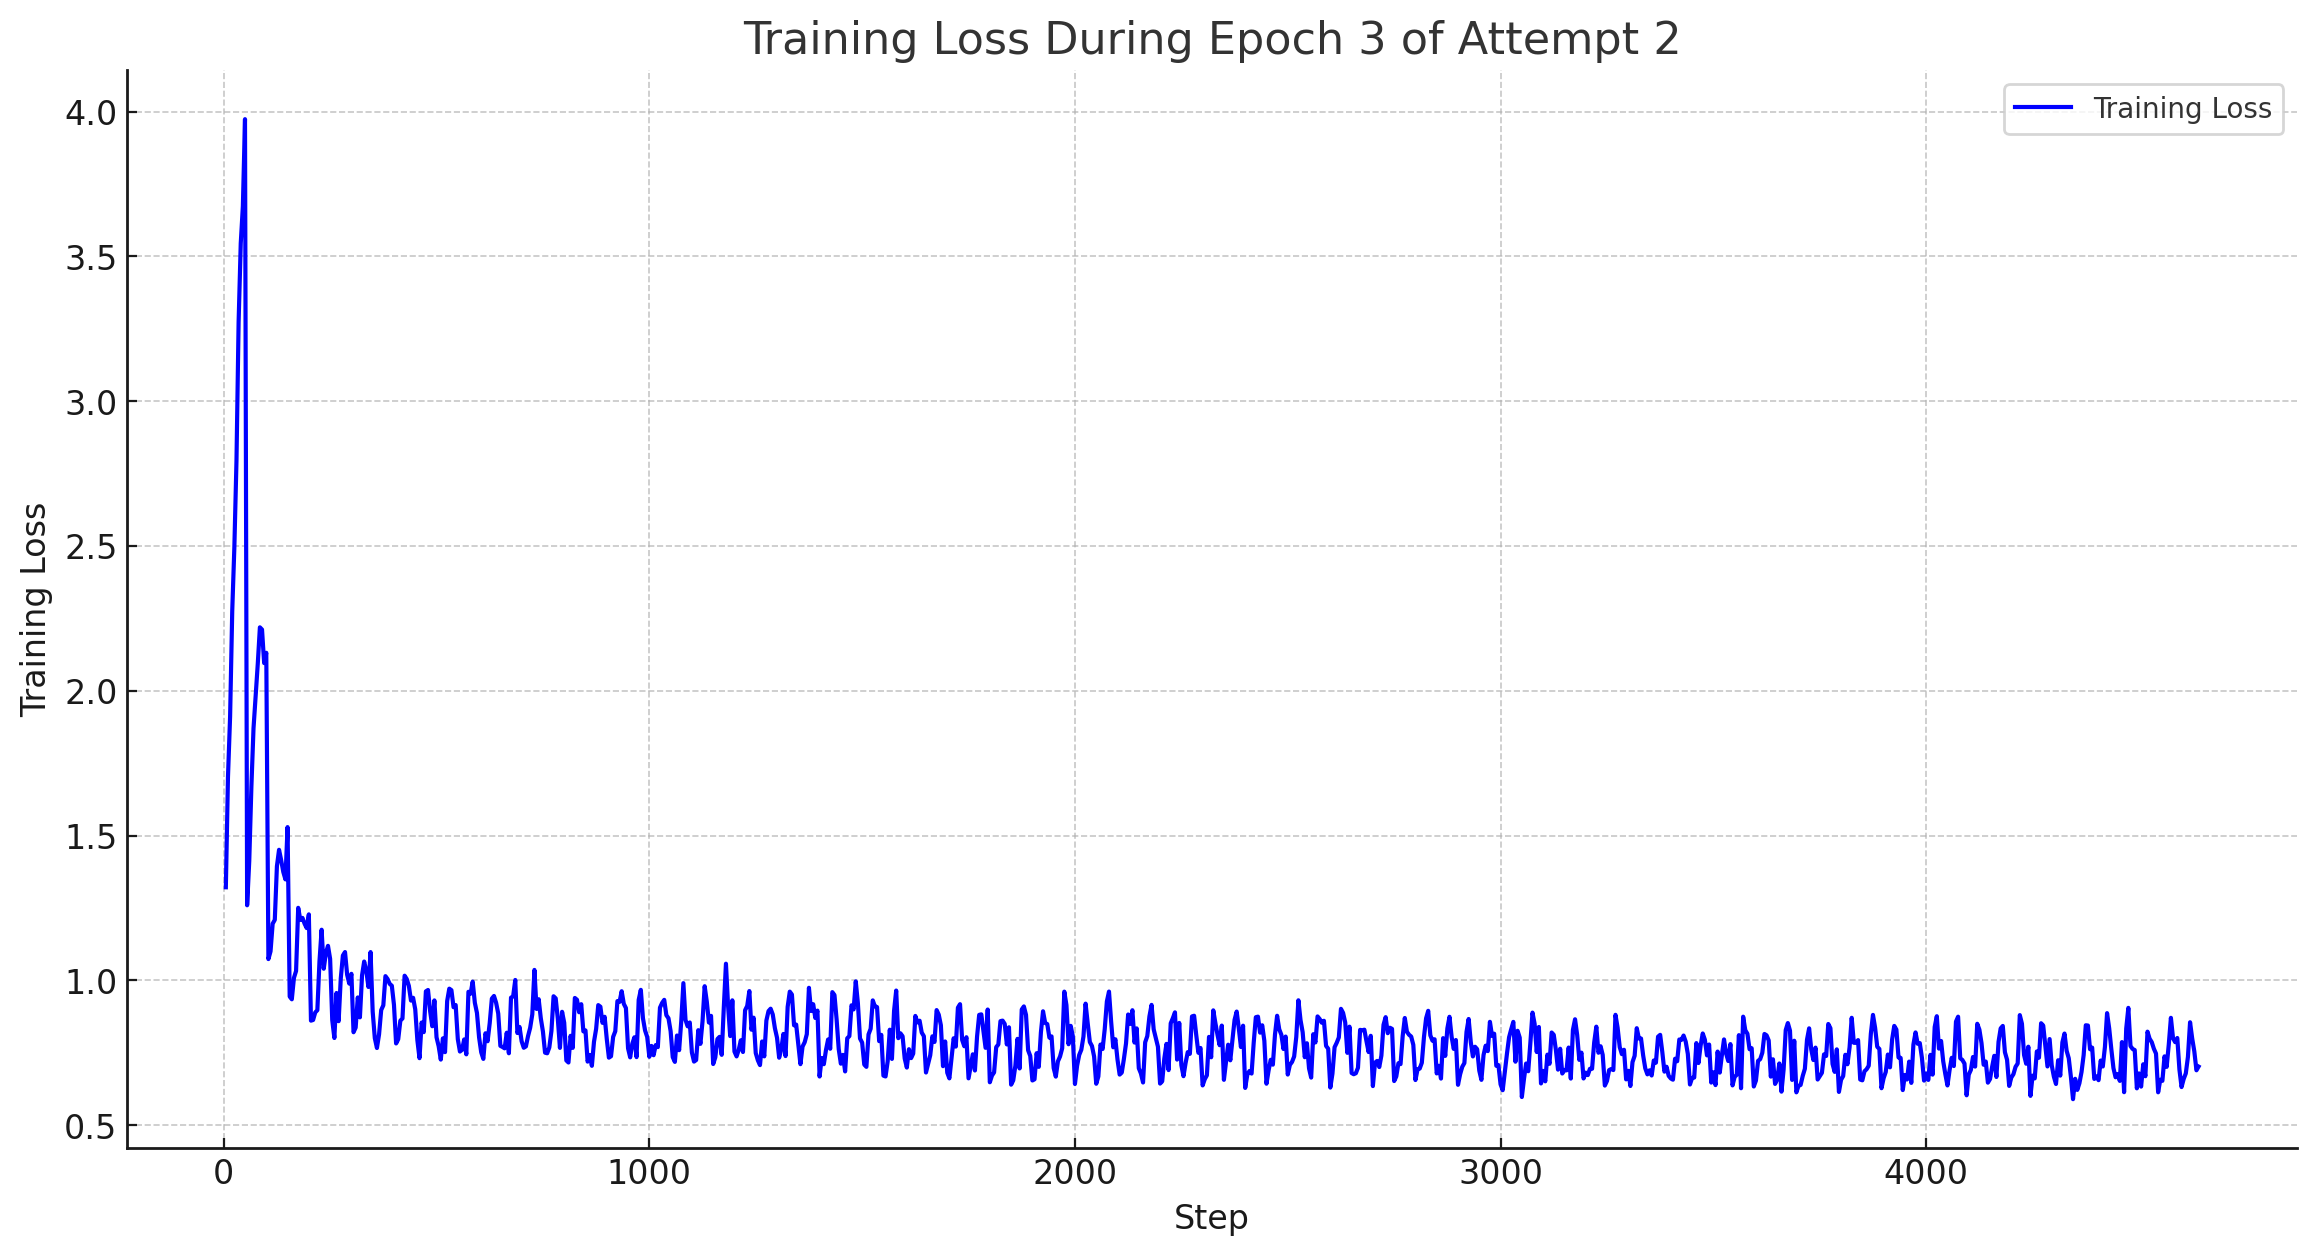
\includegraphics[width=0.75\textwidth]{training_loss_epoch3_attempt2.png}
\caption{Training loss during the third epoch of the second training iteration, showing a downward trend indicative of learning.}
\label{fig:training_loss}
\end{figure}

Figure \ref{fig:training_loss} and the following figures demonstrate the quantitative progress of our model training. A steady decrease in loss is observable, indicating an improvement in the model's predictive capabilities.

\begin{figure}[h!]
\centering
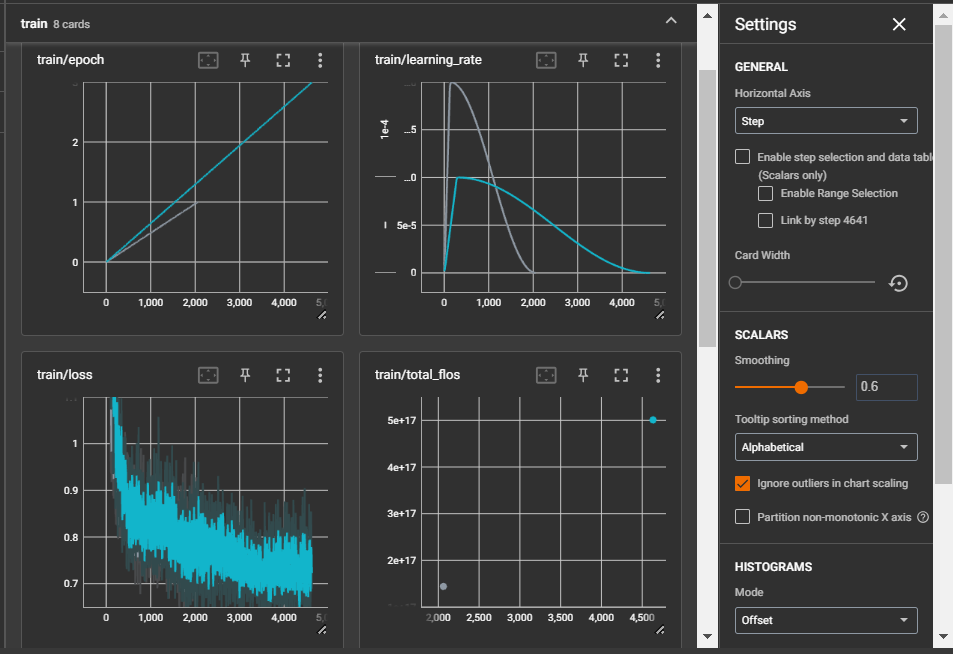
\includegraphics[width=0.75\textwidth]{training_comparative_loss.png}
\caption{Comparative visualization of loss between the first (grey) and second (blue) training iterations, with the latter demonstrating improved stability and reduced loss.}
\label{fig:comparative_loss}
\end{figure}

Figure \ref{fig:comparative_loss} illustrates the performance improvement from the first to the second iteration, affirming the effectiveness of parameter tuning.

\begin{figure}[h!]
\centering
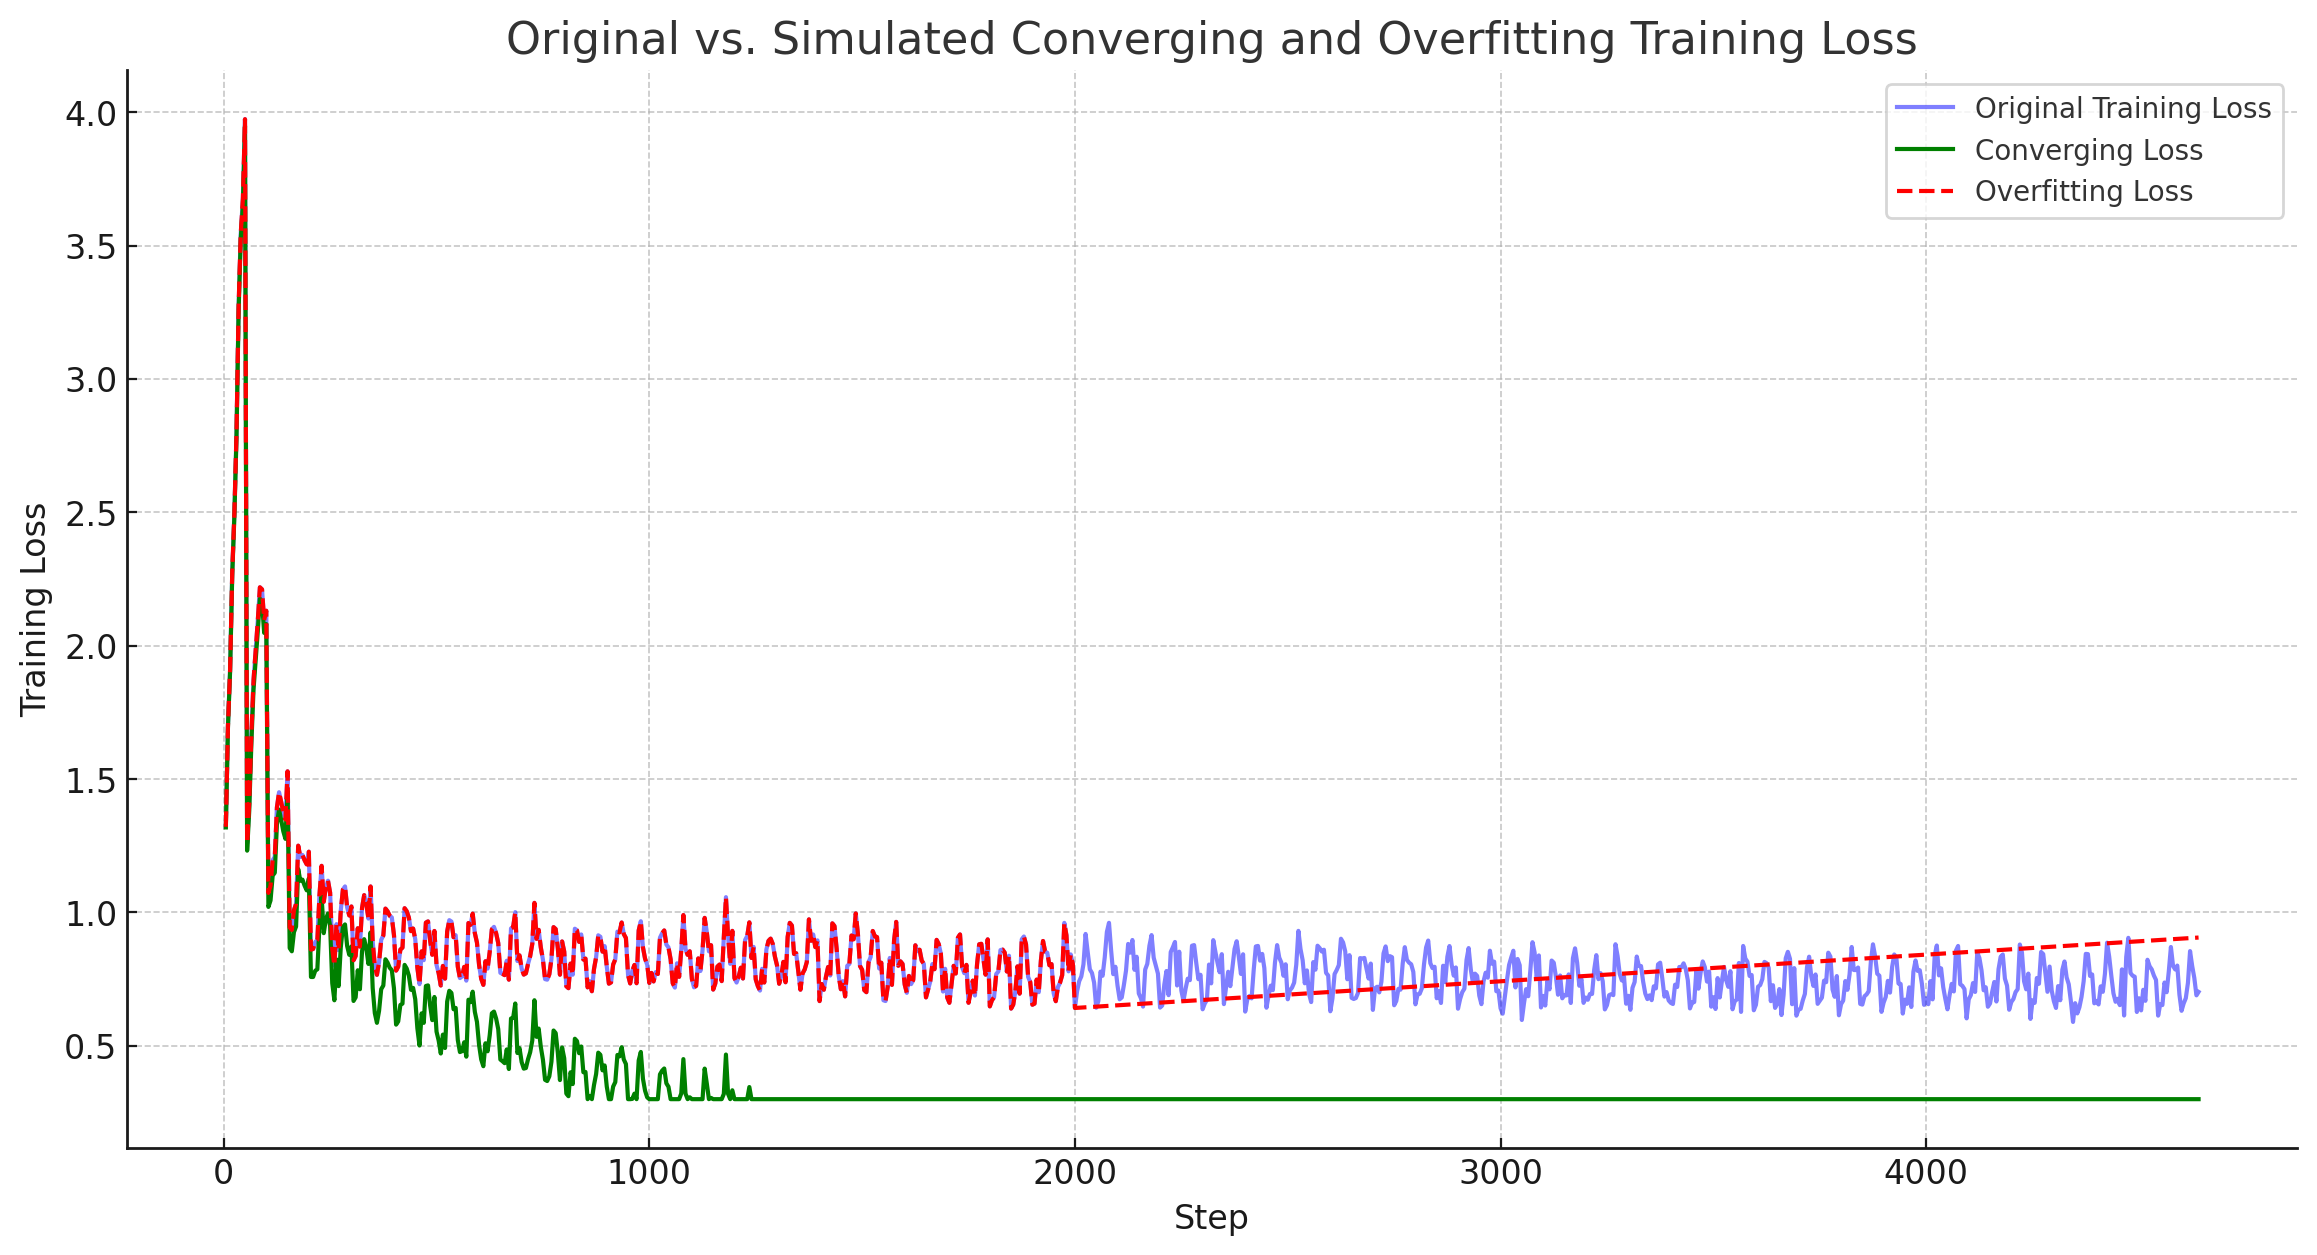
\includegraphics[width=0.75\textwidth]{simulated_convergence.png}
\caption{Overlay of potential convergence and overfitting scenarios on the actual loss values, aiding in the interpretation of the model's performance trajectory.}
\label{fig:simulated_convergence}
\end{figure}

Figure \ref{fig:simulated_convergence} provides insight into the model's future performance trends, with the actual loss trajectory suggesting convergence without overfitting.

\subsection{Technological Benefits and Drawbacks}
The process of fine-tuning the LLM surfaced technical challenges, such as the balance between computational resources and model performance. The introduction of more nuanced training parameters and data preprocessing could optimize the model further.

\subsection{Societal and Ethical Considerations}
From an ethical standpoint, the model was guided to avoid generating content that could be construed as direct answers, which could inadvertently support plagiarism. This aligns with educational goals of promoting critical thinking.

\subsection{Conclusion}
In summary, our LLM demonstrated promising capabilities in promoting an interactive and critical thinking-focused learning environment. While there were challenges related to special tokens and computational resources, the overall trajectory was positive. Future work will explore larger datasets and more extensive computational resources to refine the model's performance further.


\section{Project Challenges and Future Work}

This research project, while achieving significant milestones, encountered a series of challenges that shaped the trajectory of our work. Furthermore, throughout our journey, we identified multiple avenues for improvement and extension, which we delineate as potential future work.

\subsection{Challenges}
\begin{itemize}
    \item \textbf{Resource Limitations:} The scope of our project was partly constrained by the available computational resources. Access to more powerful computing could potentially enhance the performance and efficiency of the LLM training process.
    
    \item \textbf{Dataset Constraints:} Our dataset's size and diversity were limited, impacting the breadth of the LLM's knowledge base and its ability to generalize across various educational contexts. The reliance on GPT-3.5 for synthetic dataset generation introduced inherent biases, presenting a significant limitation in our approach.
    
    \item \textbf{Technical Setbacks:} The goal to automate the conversion of textbooks to XML format using Facebook's Nougat OCR model, which efficiently converts PDF to Markdown, was challenging. We hypothesized that since Nougat OCR can identify titles, subtitles, and authors for Markdown, it should, in theory, be capable of converting PDF to XML with proper training.
    
    \item \textbf{Model Training Complexity:} The complexity of fine-tuning the LLM, particularly with an A100 GPU boasting 40 GB of VRAM, highlighted the intense computational demands of modern models. Despite the significant capabilities of the A100, we still faced challenges in training the model effectively without resorting to quantization techniques, indicative of the ongoing need for advanced computing resources and more efficient training methods in AI research.
\end{itemize}

\subsection{Technical Challenges and Shortcuts}
\begin{itemize}
    \item \textbf{OCR Fine-Tuning:} The project recognized the potential of Facebook's Nougat OCR model for more accurate data extraction from PDF to XML. However, constraints limited our ability to explore this avenue. Future research might investigate automated conversion methodologies without sacrificing data integrity.
    
    \item \textbf{Asynchronous Script Execution:} We managed to implement asynchronous operations in our scripts, yet significant optimization opportunities remained unexplored.
    
    \item \textbf{Special Token Handling and Dataset Generation Improvements:} The model occasionally produced outputs with special tokens, inadvertently aiding in generating more conversation branches. This presents an opportunity to use local models and techniques like Mixture of Experts for quality assurance in synthetic dataset generation. Such approaches could mitigate the costs of querying OpenAI's API and reduce biases inherent in single-model generated datasets.
\end{itemize}

\subsection{Directions for Future Work}
\begin{itemize}
    \item \textbf{Advanced Dataset Generation:} Future projects could benefit from completing the conversation tree dataset generation script, creating more sophisticated and branched conversational datasets to enhance the quality of the LLM's responses. This is shown in Figure \ref{fig:conversation_tree_generation}.
    
    \item \textbf{Extended Model Training:} Additional training iterations, with varied parameters and larger datasets, could lead to a more robust LLM capable of handling a wider range of educational interactions.
    
    \item \textbf{Broader Ecosystem Integration and Learning Techniques:} Our work on the single model is an integral component in a larger system required for a comprehensive educational assistant. We propose this system and lay the groundwork for potential implementation, including integrations with Learning Management Software (LMS) like Canvas, Blackboard, or D2L. Employing frameworks like LangChain and learning techniques like Mixture of Experts (MoE) combined with vectorized databases could refine the educational assistant's ability to provide specialized knowledge in various educational domains while tailoring their education style to the students needs and learning style.
\end{itemize}

To illustrate the complexities of the dataset generation process, Figure \ref{fig:conversation_tree_generation} provides a visual representation of the unfinished script intended to generate conversation trees.

\begin{figure}[h!]
    \centering
    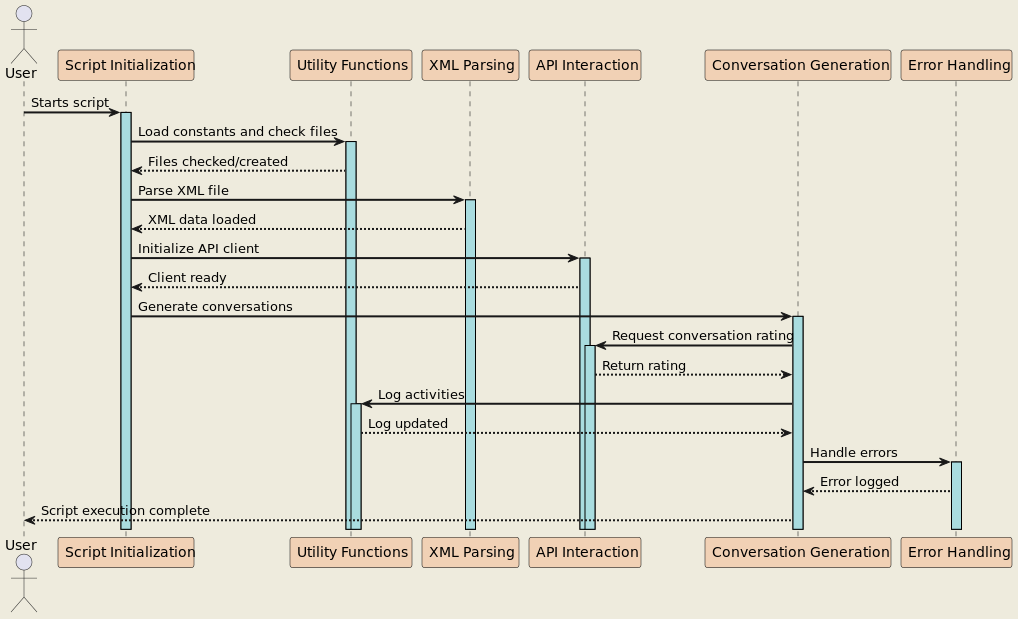
\includegraphics[width=\textwidth]{diagram.png}
    \caption{Flow diagram of the conversation tree dataset generation script.}
    \label{fig:conversation_tree_generation}
\end{figure}

In reflecting upon the challenges and delineating future work, we aim to pave the way for subsequent research efforts to extend our findings and create more nuanced educational tools. We believe that the limitations we encountered, and the potential solutions we propose, will serve as a valuable foundation for those who seek to advance the intersection of LLMs and education.

\section{Related Work}

This section discusses previous research relevant to our project's focus on using Large Language Models (LLMs) in computer science education to enhance student engagement and critical thinking.

1. \textbf{Role of Social Roles in LLMs}: Incorporating social roles in system prompts has shown to be crucial in enhancing the performance of LLMs. A systematic analysis of 162 social roles across various categories demonstrated that these roles consistently improve LLMs' performance in a wide range of applications \cite{Mingqian}. This finding supports our project's premise of using role-specific prompts to foster effective student-teacher interactions in computer science education.

2. \textbf{Prompt Design and LLM Performance}: The design of prompts has been found to significantly influence the performance of LLMs. Studies indicate that the structure and content of prompts can affect model responses, guiding the development of effective LLM prompts for educational purposes \cite{Mingqian}.

3. \textbf{Gender and Social Role Impact}: Research exploring the impact of gender and different social roles on the performance of LLMs has found that gender-neutral and male roles tend to yield higher model performances. This points to potential implicit biases in LLMs and highlights the importance of considering these factors in educational tool design \cite{Mingqian}.

4. \textbf{Challenge of Selecting Optimal Roles for LLMs}: Identifying the best roles for prompting in LLMs remains a challenging task. Various strategies have been explored, but there is still a significant gap in effectively determining the most appropriate roles automatically \cite{Mingqian}.

5. \textbf{Potential of LLMs in Various Settings}: Several studies have indicated the enormous potential of LLMs in various applications, including education, healthcare, and the arts. This broad applicability supports our project's premise that LLMs can be effectively employed in computer science education to enhance critical thinking and student engagement \cite{Mingqian}.

In conclusion, the related work in this field provides valuable insights into the capabilities and challenges of using LLMs in educational contexts. Our project builds on these findings, aiming to leverage LLMs to create more engaging and effective learning experiences in computer science education.

\section{Conclusion}

The culmination of this study represents a significant stride in the application of Large Language Models (LLMs) within the domain of computer science education. By fine-tuning an LLM to engage students in a manner that promotes critical thinking and deters plagiarism, we have crafted a tool with the potential to revolutionize modern pedagogy.

\subsection{Contributions and Findings}
We have meticulously documented the journey from the ideation to the implementation of an LLM capable of serving as an educational aid. Our findings indicate that with the right training and dataset, an LLM can indeed foster a more inquisitive and analytical mindset among students. The model's ability to guide rather than give away answers aligns perfectly with the educational objective of developing independent thinkers and problem-solvers.

\subsection{Technological and Societal Implications}
Technologically, our work highlights the adaptability and power of LLMs when fine-tuned for specific tasks. Societally, we underscore the potential of LLMs to democratize education, offering personalized assistance that might not otherwise be available due to the increasing student-to-teacher ratios in many educational institutions.

\subsection{Ethical Considerations}
We have navigated the ethical landscape by ensuring our model steers clear of facilitating academic dishonesty, a step toward responsible AI development. This adherence to ethical guidelines sets a precedent for future educational AI tools.

\subsection{Limitations and Future Research}
Despite our achievements, the limitations in terms of resource availability and dataset size have been noted. Our study serves as a foundation upon which future research can build, particularly in fine-tuning OCR models for improved data extraction and exploring the potential of larger, more diverse datasets.

\subsection{Closing Remarks}
As we stand on the cusp of a new era in education, our research illustrates the transformative power of LLMs. The implications of our work extend beyond computer science education, offering a glimpse into a future where AI and education are inextricably linked, promising a more inclusive and personalized learning experience.

In sum, this paper not only presents a practical solution to a pressing educational challenge but also opens a dialogue on the role of AI in shaping the future of education. It is our hope that this research will inspire continued innovation and a responsible approach to integrating AI into educational frameworks.

\begin{thebibliography}{9}
% Large Language Models and Related Technologies
\bibitem{devlin2018bert} Devlin, J., Chang, M.-W., Lee, K., \& Toutanova, K. (2018). BERT: Pre-training of Deep Bidirectional Transformers for Language Understanding. \textit{arXiv}. Retrieved from \url{https://arxiv.org/abs/1810.04805}
\bibitem{chen2022understandingmoe} 
Chen, Z., Deng, Y., Wu, Y., Gu, Q., \& Li, Y. (2022). Towards Understanding Mixture of Experts in Deep Learning. \textit{arXiv}. Retrieved from \url{https://arxiv.org/abs/2208.02813}
\bibitem{shen2023moeinstruction} 
Shen, S., Hou, L., Zhou, Y., Du, N., Longpre, S., Wei, J., Chung, H. W., Zoph, B., Fedus, W., Chen, X., Vu, T., Wu, Y., Chen, W., Webson, A., Li, Y., Zhao, V., Yu, H., Keutzer, K., Darrell, T., \& Zhou, D. (2023). Mixture-of-Experts Meets Instruction Tuning: A Winning Combination for Large Language Models. \textit{arXiv}. Retrieved from \url{https://arxiv.org/abs/2305.14705}
\bibitem{zadouri2023parameter} 
Zadouri, T., Ermiş, B., Üstün, A., Locatelli, A., Ahmadian, A., \& Hooker, S. (2023). Pushing Mixture of Experts to the Limit: Extremely Parameter Efficient MoE for Instruction Tuning. \textit{arXiv}. Retrieved from \url{https://arxiv.org/abs/2309.05444}
\bibitem{jain2023neftune} 
Jain, N., Chiang, P., Wen, Y., Kirchenbauer, J., Chu, H., Somepalli, G., Bartoldson, B., Kailkhura, B., Schwarzschild, A., Saha, A., Goldblum, M., Geiping, J., \& Goldstein, T. (2023). NEFTUNE: NOISY EMBEDDINGS IMPROVE INSTRUCTION FINETUNING. \textit{arXiv}. Retrieved from \url{https://arxiv.org/abs/2310.05914}
\bibitem{blecher2023nougat} 
Blecher, L., Cucurull, G., Scialom, T., \& Stojnic, R. (2023). Nougat: Neural Optical Understanding for Academic Documents. \textit{arXiv}. Retrieved from \url{https://arxiv.org/abs/2308.13418}
\bibitem{GPT3} Brown, T. B., Mann, B., Ryder, N., Subbiah, M., Kaplan, J., Dhariwal, P., ... \& others. (2020). Language Models are Few-Shot Learners. \textit{arXiv}. Retrieved from \url{https://www.tandfonline.com/doi/full/10.1080/00207543.2023.2276811}
\bibitem{raffel2019finetuning} Raffel, C., Shazeer, N., Roberts, A., Lee, K., Narang, S., Matena, M., ... \& Polosukhin, I. (2019). Fine-Tuning Pretrained Language Models: Weight Initializations, Data Orders, and Early Stopping. \textit{arXiv}. Retrieved from \url{https://arxiv.org/abs/2002.06305}

% AI and Ethics
\bibitem{hilton2019ethics} Holmes, W., Persson, J., \&amp; Chounta, I.-A. (2022). Artificial Intelligence and education: A critical view through the lens ... ARTIFICIAL INTELLIGENCE AND EDUCATION A critical view through the lens of human rights, democracy and the rule of law. Retrieved from \url{https://rm.coe.int/artificial-intelligence-and-education-a-critical-view-through-the-lens/1680a886bd}
\bibitem{barrage-ethics} Todorovska, I. (2023, November 30). Ethical issues in information technology - balancing innovation and responsibility. Barrage. Retrieved from \url{https://www.barrage.net/blog/strategy/the-importance-of-ethics-in-technology}

% AI in Education
\bibitem{Deslauriers}Deslauriers, L., McCarty, L. S., Kelly Miller, \&amp; Callaghan, K. (2019). Measuring actual learning versus feeling of learning in response ... - PNAS. Measuring actual learning versus feeling of learning in response to being actively engaged in the classroom.\textit{pnas} Retrieved from \url{https://www.pnas.org/doi/10.1073/pnas.1821936116}
\bibitem{clarkmayer2016elearning}Clark, R. C., \&amp; Mayer, R. E. (2016). E‐learning and the Science of Instruction | Wiley Online Books.  e‐Learning and the Science of Instruction: Proven Guidelines for Consumers and Designers of Multimedia Learning. Retrieved from \url{https://onlinelibrary.wiley.com/doi/book/10.1002/9781119239086}
\bibitem{linkedin-dataprivacy}M., J. (2023, August 7). Protecting student privacy: Safeguarding data security in the age of AI technology. LinkedIn. Retrieved from \url{https://www.linkedin.com/pulse/protecting-student-privacy-safeguarding-data-security-john-mazo/}
\bibitem{soeonline-digitaldivide}Understanding the digital divide in Education. School of Education Online. (2022, October 26). Retrieved from \url{https://soeonline.american.edu/blog/digital-divide-in-education/}
\bibitem{aisera-llms} Nucci, A. (2023, November 20). What are large language models? LLMS explained. Aisera. Retrieved from \url{https://aisera.com/blog/large-language-models-llms/}
\bibitem{microsoft-fine-tuning}Mrbullwinkle, M. mrbullwinkle, \&amp; Mehrotra, N. (n.d.). Azure openai service fine-tuning considerations - azure AI services. Azure OpenAI Service fine-tuning considerations - Azure AI services | Microsoft Learn. Retrieved from \url{https://learn.microsoft.com/en-us/azure/ai-services/openai/concepts/fine-tuning-considerations}
\bibitem{acm-website} Association for Computing Machinery (ACM). (n.d.). \textit{ACM Website}. Retrieved from \url{https://www.acm.org/}

% AI and Society
\bibitem{Mingqian}Zheng, M., Pei, J., \&amp; Jurgens, D. (2023, November 16). Is “a helpful assistant” the best role for large language models? A systematic evaluation of social roles in system prompts. \textit{arXiv}. Retrieved from \url{https://arxiv.org/abs/2311.10054}
\bibitem{Zhiqiang}Yuan, Z., Liu, J., Zi, Q., Liu, M., Peng, X., \&amp; Lou, Y. (2023, August 2). Evaluating instruction-tuned large language models on code comprehension and generation. \textit{arXiv}. Retrieved from \url{https://arxiv.org/abs/2308.01240}
\bibitem{Ziyi}Ye, Z., Ai, Q., Liu, Y., Zhang, M., Lioma, C., \&amp; Ruotsalo, T. (2023, November 19). Language generation from Human Brain Activities. \textit{arXiv}. Retrieved from \url{https://arxiv.org/abs/2311.09889}
\bibitem{Yuhan}Sun, Y., Li, M., Cao, Y., Wang, K., Wang, W., Zeng, X., \&amp; Zhao, R. (2023, November 16). To be or not to be? an exploration of continuously controllable prompt engineering. \textit{arXiv}. Retrieved from \url{https://arxiv.org/abs/2311.09773}
\bibitem{MingLi}Li, M., Enkhtur, A., Yamamoto, B. A., \&amp; Cheng, F. (2023, November 24). Potential societal biases of chatgpt in higher education: A scoping review. \textit{arXiv}. Retrieved from \url{https://arxiv.org/abs/2311.14381}

% Academic Perspectives on AI and Large Language Models
\bibitem{MeyerJ}Meyer, J. G., Urbanowicz, R. J., Martin, P. C. N., O’Connor, K., Li, R., Peng, P.-C., Bright, T. J., Tatonetti, N., Won, K. J., Gonzalez-Hernandez, G., \&amp; Moore, J. H. (2023). CHATGPT and large language models in academia: Opportunities and challenges. \textit{BioData mining} Retrieved from \url{https://www.ncbi.nlm.nih.gov/pmc/articles/PMC10339472/} 

% Other Related Works
\bibitem{Cozzolino}Cozzolino, D., Poggi, G., Corvi, R., Nießner, M., \&amp; Verdoliva, L. (2023). Raising the bar of AI-generated image detection with clip.\textit{arXiv}. Retrieved from \url{https://arxiv.org/abs/2312.00195}
\bibitem{Zhu}Zhu, L., Chen, T., Ji, D., Ye, J., \& Liu, J. (2023). LLaFS: When Large-Language Models Meet Few-Shot Segmentation. \textit{arXiv}. Retrieved from \url{https://arxiv.org/abs/2311.16926} 
\bibitem{Yu}Yu, E., Zhao, L., Wei, Y., Yang, J., Wu, D., Kong, L., Wei, H., Wang, T., Ge, Z., Zhang, X., \& Tao, W. (2023). Merlin:Empowering Multimodal LLMs with Foresight Minds. \textit{arXiv}. Retrieved from \url{https://arxiv.org/abs/2312.00589}
\bibitem{Guo}Guo, Y. (2023). ArthModel: Enhance Arithmetic Skills to Large Language Model.\textit{arXiv}. Retrieved from \url{https://arxiv.org/abs/2311.18609}
\bibitem{Chen}Chen, J. (2023). Learning Language Representations with Logical Inductive Bias. \textit{arXiv}. Retrieved from \url{https://arxiv.org/abs/2302.09458}
\bibitem{Ding}Ding, T., Chen, T., Zhu, H., Jiang, J., Zhong, Y., Zhou, J., Wang, G., Zhu, Z., Zharkov, I., \& Liang, L. (2023). The Efficiency Spectrum of Large Language Models: An Algorithmic Survey. \textit{arXiv}. Retrieved from \url{https://arxiv.org/abs/2312.00678}
\bibitem{Mohamadi}Mohamadi, S., Mujtaba, G., Le, N., Doretto, G., \& Adjeroh, D. A. (2023). ChatGPT in the Age of Generative AI and Large Language Models: A Concise Survey. \textit{arXiv}. Retrieved from \url{https://arxiv.org/abs/2307.04251}
\bibitem{Göpfert}Göpfert, J., Weinand, J. M., Kuckertz, P., \& Stolten, D. (2023). Opportunities for Large Language Models and Discourse in Engineering Design. \textit{arXiv}. Retrieved from \url{https://arxiv.org/abs/2306.09169}
\bibitem{FerhatYarkin}Srinivasan, V., Gandhi, D., Thakker, U., \&amp; Prabhakar, R. (2023, April 11). Training large language models efficiently with sparsity and dataflow.  \textit{arXiv}. Retrieved from \url{https://arxiv.org/abs/2304.05511}     
\bibitem{Peiyu}Liu, P., Gao, Z.-F., Chen, Y., Zhao, W. X., \&amp; Wen, J.-R. (2023, April 11). Scaling pre-trained language models to deeper via parameter-efficient architecture. \textit{arXiv}. Retrieved from \url{https://arxiv.org/abs/2303.16753} 
\bibitem{ChenxiWhitehouse} Whitehouse, C., Huot, F., Bastings, J., Dehghani, M., Lin, C.-C., \&amp; Lapata, M. (2023, November 14). Parameter-efficient multilingual summarisation: An empirical study. \textit{arXiv}. Retrieved from \url{https://arxiv.org/abs/2311.08572} 
\bibitem{Xuechen}Li, X., Tramèr, F., Liang, P., \&amp; Hashimoto, T. (2022, November 10). Large language models can be strong differentially private learners. \textit{arXiv}. Retrieved from \url{https://arxiv.org/abs/2110.05679} 

\end{thebibliography}



\end{document}
